\documentclass[11pt, oneside]{article}
\usepackage{geometry}
\geometry{letterpaper}

%%% Diagram drawing
\usepackage{tikz}
\usetikzlibrary{arrows,automata,calc,shapes, positioning}

%% math
\newcommand{\set}[1]{\{#1\}}

%% LTLf/LDLf
\let\vphi\varphi % alternate phi, which I'll be using a lot
\newcommand{\di}[1]{\langle#1\rangle} % 'diamond' For LDL modalities
\newcommand{\sq}[1]{[#1]} % 'square'
\newcommand{\luntil}{\ \mathcal{U}\ }
\newcommand{\lalways}{\mathcal{G}}
\newcommand{\leventually}{\mathcal{F}}
\newcommand{\lnext}{\circ\,}
\newcommand{\prog}{\Pi}
\newcommand{\A}{\mathnormal{A}}
\newcommand{\prop}{\mathcal{P}}
\newcommand{\actions}{\mathcal{A}}
\newcommand{\fin}[1]{#1$_f$}
\newcommand{\ltlf}{LTL$_f\ $}
\newcommand{\ldlf}{LDL$_f\ $}

\begin{document}

\newcommand{\ldlfa}{LDL$_f$}
\newcommand{\ldlfb}{LDL$_f\,$}
\ldlf. \ldlf blah.
\\\ldlfa. \ldlfa blah.
\\\ldlfb. \ldlfb blah.

{\newcommand{\lab}{$\lnext$}
\begin{figure}
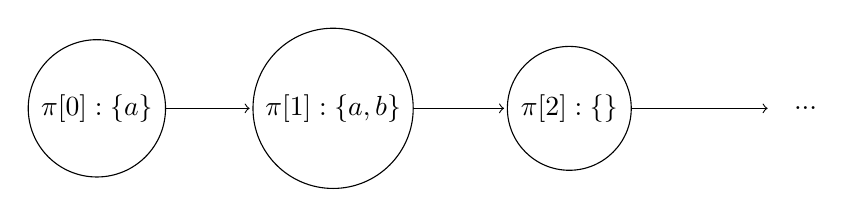
\begin{tikzpicture}[shorten >=1pt,node distance=3cm,on grid,auto]
   \node[state] (q1)   {$\pi[0]: \set{a}$};
   \node[state] (q2) [right=of q1] {$\pi[1]: \set{a,b}$};
   \node[state] (q3) [right=of q2] {$\pi[2]: \set{}$};
   \node[state, draw=none] (q4) [right=of q3] {...};
    \path[->]
    (q1) edge node {\lab} (q2)
    (q2) edge node {\lab} (q3)
    (q3) edge node {\lab} (q4);

\end{tikzpicture}
    \caption{Diagram of an infinite trace\label{fig:inf_trace_diagram}}
\end{figure}
}


\end{document}
